
\documentclass{beamer}
\usepackage{lmodern}
\usepackage{wasysym}
\usepackage{graphicx}
\usepackage{listings}
\usepackage[T1]{fontenc}
\usepackage[utf8]{inputenc}
\date{\today}
\lstdefinestyle{basic}{
    captionpos=t,%
    basicstyle=\footnotesize\ttfamily,%
    numberstyle=\tiny,%
    numbers=left,%
    stepnumber=1,%
    frame=single,%
    showspaces=false,%
    showstringspaces=false,%
    showtabs=false,%
    %
    keywordstyle=\color{blue},%
    identifierstyle=,%
    commentstyle=\color{gray},%
    stringstyle=\color{magenta}%
}
\usecolortheme{default}
\setbeamertemplate{navigation symbols}{}
\setbeamertemplate{navigation symbols}{}
\setbeamertemplate{blocks}[rounded][shadow=true]
\setbeamercolor{block title}{bg=blue!20!white}
\setbeamercolor{block body}{bg=blue!5!white}

\begin{document}





% more spaces
\newlength{\wideitemsep}
\setlength{\wideitemsep}{\itemsep}
\addtolength{\wideitemsep}{2pt}
\let\olditem\item
\renewcommand{\item}{
    \setlength{\itemsep}{\wideitemsep}
    \olditem
}

\begin{frame}
    \title{Embedding the Petersen Graph on the Cross Cap}
    \author{Julius Plenz / Martin Zänker}
    \date{2013-12-16}
    \titlepage
\end{frame}

\begin{frame}
 \frametitle{Petersen Graph}
  


\begin{itemize}
  \item Special Case of the Kneser Graph ($KG_{5,2}$)
  \item Chromatic number of $KG_{n,k}$ is $n - 2k + 2$
  \item Will have intersecting edges in any realization in $\mathbb{R}^2$
  \item Smallest bridgeless cubic graph with no three-edge-coloring
\end{itemize}

\begin{block}{Donald Knuth about the Petersen Graph}
[The Petersen Graph is] a remarkable configuration that serves as a
counterexample to many optimistic predictions about what might be true for
graphs in general.
\end{block}

  
 \end{frame}
\begin{frame}
 \frametitle{The Petersen Graph and a Three-Coloring}
  


\begin{center}
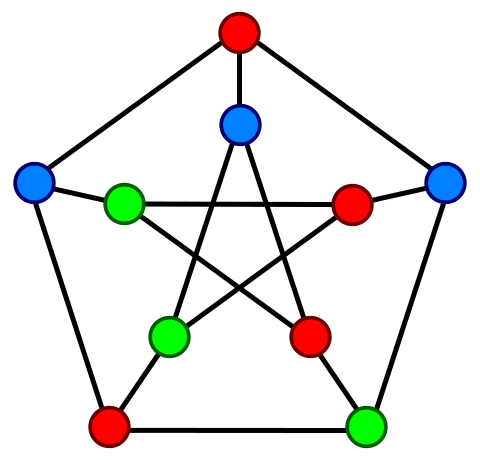
\includegraphics[width=0.7\textwidth]{petersen-graph.png}
\end{center}

\hfill\footnotesize{Image: Wikipedia / Public Domain}

  
 \end{frame}
\begin{frame}
 \frametitle{The Cross Cap}
  


\begin{itemize}
  \item Homeomorphic to $\mathbb{R}P^2$, the real projective plane
  \item Obtained by identifying border points of the a two-cover of $D^2$
  \item Cannot be realized without self-intersection in $\mathbb{R}^3$
\end{itemize}

\begin{center}
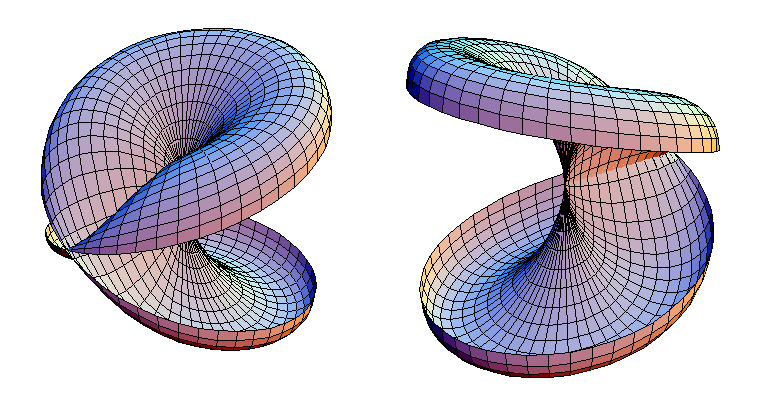
\includegraphics[width=0.6\textwidth]{CrossCapSlicedOpen.PNG}
\end{center}
\hfill\footnotesize{Image: Wikimedia Commons / GNU FDL}

  
 \end{frame}
\begin{frame}
 \frametitle{Plan}
  


\begin{itemize}
  \item Research graph-theoretical properties of the Petersen Graph
  \item Research topological properties of the Cross Cap
  \item Create a realization of the Cross Cap in Maya
  \item Embed the Petersen Graph with a suitable coloring in the Cross Cap realization
  \item Create an insightful animation of the embedding
\end{itemize}

  
 \end{frame}


\end{document}

